\documentclass{article}

\usepackage{amsmath, amsthm, amssymb, amsfonts}
\usepackage{thmtools}
\usepackage{graphicx}
\usepackage{setspace}
\usepackage{geometry}
\usepackage{float}
\usepackage{hyperref}
\usepackage[utf8]{inputenc}
\usepackage[english]{babel}
\usepackage{framed}
\usepackage[dvipsnames]{xcolor}
\usepackage{tcolorbox}
\usepackage{mathrsfs}
\usepackage{bbm}
\usepackage{dsfont} % For the indicator function \mathds{1}

\colorlet{LightGray}{White!90!Periwinkle}
\colorlet{LightOrange}{Orange!15}
\colorlet{LightGreen}{Green!15}
\colorlet{LightBlue}{Blue!15}

\newcommand{\HRule}[1]{\rule{\linewidth}{#1}}

\declaretheoremstyle[name=Theorem,]{thmsty}
\declaretheorem[style=thmsty,numberwithin=section]{theorem}
\tcolorboxenvironment{theorem}{colback=LightGray}

\declaretheoremstyle[name=Proposition,]{prosty}
\declaretheorem[style=prosty,numberlike=theorem]{proposition}
\tcolorboxenvironment{proposition}{colback=LightOrange}

\declaretheoremstyle[name=Definition,]{prcpsty}
\declaretheorem[style=prcpsty,numberlike=theorem]{definition}
\tcolorboxenvironment{definition}{colback=LightGreen}

\declaretheoremstyle[name=Remark,]{prosty}
\declaretheorem[style=prosty,numberlike=theorem]{remark}
\tcolorboxenvironment{remark}{colback=LightBlue}

\setstretch{1.2}
\geometry{
    textheight=9in,
    textwidth=5.5in,
    top=1in,
    headheight=12pt,
    headsep=25pt,
    footskip=30pt
}

% ------------------------------------------------------------------------------

\begin{document}

% ------------------------------------------------------------------------------
% Cover Page and ToC
% ------------------------------------------------------------------------------

\title{ \normalsize \textsc{}
		\\ [2.0cm]
		\HRule{1.5pt} \\
		\LARGE \textbf{\uppercase{MATH 412: Statistical Machine Learning}
		\HRule{2.0pt} \\ [0.6cm] \LARGE{Rafiki's Notes} \vspace*{10\baselineskip}}
		}
\date{}
\author{\textbf{Rafael Barroso} \\ 
		Ingenierie Mathematique \\
		École Polytechnique Fédérale de Lausanne \\
		\today}

\maketitle
\newpage

\tableofcontents
\newpage

% ------------------------------------------------------------------------------

\section{Supervised Learning Basics} \label{sec:sup-learing-basics}
In this area of machine learning, we try to understand certain relations beween input-output data. If such relations are established, we then wish to generalize for new \textit{unseen} data.
Things start getting even jucier whenever we wish to take decisions based on new data, resulting in a more generalized task. In this section we explore the formalization provided by Prof. Obozinski.

\begin{enumerate}
    \item \textbf{We have:}
    \begin{itemize}
        \item Data: $\mathcal{D}_n := \left\{ (x_0,y_0), \ldots, (x_n,y_n) \right\}$
        \item i.e. tuples of the form $(x_i, y_i)$
        \item $x_i:=$ input; $y_i:=$ output
    \end{itemize}

    \item \textbf{We want:}
    \begin{itemize}
        \item Given $\mathcal{D}_n$, learn relations of the $x_i$'s with the corresponding $y_i$'s such that we may infer something about a new unseen $y'$ given $x'$.
    \end{itemize}
\end{enumerate}

We now define the two types of tasks cosidered inside supervised learning (amongst others).

\begin{definition}
    A \textit{prediction} task is established to be the discovery of $y`$ (unseen) given $x`$. A \textit{decision} task on the
    other hand, focuses on producing a decision based on $(x`,y`)$ only with the data of $x`$
\end{definition}

For example, take into consideration a medical diagnosis. We have $x_i :=$ patient data i.g. $\left\{ \text{weight}_i, \text{height}_i, \ldots \right\}$; $y_i := \left\{ \text{positive}, \text{negative} \right\}$. Then, a \textbf{prediction task} 
would consist in predicting $y`$ given $x`$. A \textbf{decision task} on the other hand, would then consist on choosing how to treat patient $x`$ i.g. choosing medicine $m \in \left\{ A,B,C \right\}$ (we have to decide on $y`$ by only seeing $x`$).

\vspace{0.3cm}

We now consider the space of all possible decisions; a \textit{learning algorithm }(sometimes called \textit{learning scheme}) $\mathscr{A}$. 

\begin{definition}
    We define a learning algorithm as $$\mathscr{A}: \mathcal{D}_n \rightarrow \hat{f}$$ where $\hat{f}$ is our decision function.
\end{definition}

Obviously we want $\hat{f}$ to be ``good'' (otherwise, \textit{nos estamos haciendo pendejos}). Hence, we must define what it means for $\hat{f}$ to be ``good'' i.e. what we want from $\hat{f}$. 

\begin{definition}
    Let $\mathcal{X}$ be the input space, then, a decision function is defined as $$f:\mathcal{X} \rightarrow \mathcal{A}^{\mathcal{X}}$$ Note that the input space $\mathcal{X}$ is the space of all $x_i$`s.
\end{definition}

Ideally, as stated before, we want a ``good'' function (i.e. decision function) $f$ such that $f(x) \in \mathcal{A}^{\mathcal{X}}$ is ``good'' when compared to an unseen $y$. This means that $f(x)$ must be an accurate prediction of $y$ and it has
the \textbf{smallest possible cost} whenever $y$ occurrs. So, we compute the \textit{loss function} $l$.

\begin{definition}
    Let $\mathcal{Y}$ be the space of all possible outcomes, then $$l:\mathcal{A}^{\mathcal{X}} \times \mathcal{Y} \rightarrow \mathbb{R}$$ defined by $(f(x)=a,y) \mapsto l(a,y)$. Note that this function meassures the cost of taking decision $f$ whenever $y$ occurrs i.e. the \textit{risk}.
\end{definition}

\begin{remark}
    Note that all the above definitions boil down to the fact that we're trying to design a `good' learning algorithm $\mathscr{A}$ that produces $\hat{f}$ in such a way that the risk is minimized. We formalize the definition of a learning algorithm as follows
    $$\mathscr{A}: \left(\mathcal{X} \times \mathcal{Y} \right)^{n} \rightarrow \mathcal{A}^{\mathcal{X}} \text{ given by } \mathcal{D}_n \mapsto \hat{f}$$ Throughout the lecture, unless stated otherwise, we assume that the data is generated by a stochastic process and
    done so i.i.d. as random variables i.e. $(X_i, Y_i)$.
\end{remark}

Because of the fact that this is a statistics class, we'll start getting into the \textit{deets} using much more of their language (statisticians have a fetish for fancy language and syntax). Hence we would like to define what the \textit{expected cost} of takin decision $f$ as the risk $\mathcal{R}$.

\begin{definition}
    We define the risk as follows $$\mathcal{R}(f) \text{ :}= \mathbb{E}\big[l(a,Y) \big] \text{. If  } \exists f^* \in \mathcal{A}^{\mathcal{X}} : \mathcal{R}(f^*)=\text{ inf}_{f \in \mathcal{A}^{\mathcal{X}}} \mathcal{R}(f)$$ then, that $f^*$ is our juicy function we're looking for! statisticians call it the
    \textit{target} function. Now, the \textit{conditional risk} of taking $f$ as an action given $x$ has happened is defined as $$\mathcal{R}(f(x)=a|x) = \mathbb{E}\big[l(a,Y) | X = x \big] = \int l(a,y) dP_{Y|X}(y|x)$$ 
\end{definition}

Note that $dP_{Y|X}(y|x)$ just means we're integrating over the conditional distribution of $Y$ given $X=x$. To simplify further (and remark the fetish statisticians posse), this just means that we're taking average the loss over all possible outcomes of $Y$, weighted by how likely they are given $X=x$.

\begin{remark}
    Note that $$\mathbb{E}\big[ \mathcal{R}(f(X)|X) \big] = \mathbb{E}\big[ \mathbb{E}\big[l(f(X),Y) | X = x \big]\big]=\mathbb{E} \big[l(f(X),Y)\big]$$ i.e. the expected value of $\mathcal{R}(f)$.
\end{remark}

We finally make the last definition of the section, since we're interested in meassuring risks we shall compute the \textit{excess risk} $\varepsilon(f)$ while we're at it. This number tells us how much of our risk is over the optimal ammount.

\begin{definition}
    The excess risk is given by $$\varepsilon (f) := \mathcal{R}(f) - \mathcal{R}(f^*) = \mathbb{E} \big[l(f(X),Y)\big] - \mathbb{E} \big[l(f^*(X),Y)\big]$$ $$\Rightarrow \varepsilon (f) = \mathbb{E} \big[l(f(X),Y) - l(f^*(X),Y)\big]$$
\end{definition}

This is a great book!\cite{judson2019abstract}.

\newpage

\section*{Exercise Sheet 1} \label{sec:ex01}
The following exercises are designed to reinforce the concepts introduced in this section. They provide both practice with fundamental techniques and opportunities to explore some extensions of the main results. Complete solutions are included to aid understanding and self-study.

\subsection*{Exercise 1.1: Classification from a discrete input space}

We consider a multiclass classification problem with 3 classes 
\(\mathcal{Y} = \{1,2,3\}\) for data with only a single discrete descriptor 
in \(\mathcal{X} = \{1,2,3,4\}\).

We assume that the joint probability distribution 
\(\mathbb{P}(Y = y, X = x)\), with \(X \in \mathcal{X}\) and \(Y \in \mathcal{Y}\), 
is specified by the following table:

\[
\begin{array}{c|ccc}
    & Y=1 & Y=2 & Y=3 \\ \hline
X=1 & 0.02 & 0.08 & 0.10 \\
X=2 & 0.05 & 0.40 & 0.15 \\
X=3 & 0.02 & 0.02 & 0.12 \\
X=4 & 0.02 & 0.01 & 0.01 \\
\end{array}
\]

\begin{enumerate}
    \item What is the target function \(f^*\) for the 0--1 loss?
    \item What are the values of \(f^*(x)\) for \(x = 1,2,3,4\)?
    \item What is the value of the risk for the target function?
\end{enumerate}

\textbf{Answers:}
\vspace{0.2cm}

As shown above, $f^*(x) = \arg\max_{y \in \mathcal{Y}} \mathbb{P}(Y=y | X=x)$.

\vspace{0.2cm}

Now, if $\mathcal{X} = \{1, 2, 3, 4\}$ and $\mathcal{Y} = \{1, 2, 3\}$, where $\mathbb{P}(Y=y | X=x)$ is given by a table, we find $f^**(x)$ for $x \in \mathcal{X}$. We want to find the $y$ that maximizes $\mathbb{P}(Y=y|X=x)$.
For example, if $\max_y \mathbb{P}(Y=y|X=1) = 0.1$, which occurs when $y=3$, then $f^*(1)=3$. So, for $x=1, f^*(1)=3$. If $x=2, f^*(2)=2$. For $x=3, f^*(3)=3$. For $x=4, f^*(4)=1$.

\vspace{0.2cm}

Finally, the risk is the probability of misclassification:
\[ \mathbb{P}(f^*(X) \neq Y) = \mathbb{E}[\mathds{1}_{f^*(X) \neq Y}] = \sum_{x \in \mathcal{X}} \sum_{y \in \mathcal{Y}} \mathds{1}_{f^*(x) \neq y} \mathbb{P}(X=x, Y=y) \]

\subsection*{Exercise 1.2: Recap of linear models}

Let \(y = X\beta + \varepsilon\), where \(\mathbb{E}[\varepsilon] = 0\), 
\(\mathrm{Var}(\varepsilon) = \sigma^2 I\), 
and \(X\) is a non-random full rank matrix of size \(n \times p\). 
This setup contains the Gauss--Markov assumptions of a linear model.

\begin{enumerate}
    \item Derive the least squares estimator 
    \(\hat{\beta} = (X^{\top}X)^{-1}X^{\top}y\).
    \item Show that \(\hat{\beta}\) is unbiased and that the variance of \(\hat{\beta}\) 
    is given by \(\sigma^2 (X^{\top}X)^{-1}\).
\end{enumerate}

\newpage
\textbf{Answers:}
\vspace{0.2cm}

The model is $y = X\beta + \epsilon$, with assumptions $\mathbb{E}[\epsilon]=0$ and $\text{Var}(\epsilon) = \sigma^2 I$. We assume $X$ is full rank. Note that $X^TX$ is therefore invertible (positive definite).
Since $\mathbb{E}[\epsilon]=0$, we have $\mathbb{E}[Y|X] = X\beta$.

\vspace{0.2cm}

Now, the loss function is $L(\beta) = \sum_i (y_i - x_i^T\beta)^2 = (y - X\beta)^T(y - X\beta)$.
\begin{align*}
    L(\beta) &= (y^T - (X\beta)^T)(y - X\beta) \\
    &= y^Ty - y^T X\beta - (X\beta)^T y + (X\beta)^T(X\beta) \\
    &= y^Ty - y^T X\beta - \beta^T X^T y + \beta^T X^T X \beta \\
    &= y^Ty - 2\beta^T X^T y + \beta^T X^T X \beta
\end{align*}

\vspace{0.2cm}

To find the minimum, we take the derivative with respect to $\beta$ and set it to 0.
\[ \frac{\partial L}{\partial \beta} = -2X^T y + 2X^T X \beta \]
Setting to 0:
\[ -2X^T y + 2X^T X \beta = 0 \implies X^T X \beta = X^T y \implies \hat{\beta} = (X^T X)^{-1} X^T y \]
Now, let's find the expectation of the estimator $\hat{\beta}$ to check for bias.
\begin{align*}
    \mathbb{E}[\hat{\beta}] &= \mathbb{E}[(X^T X)^{-1} X^T y] \\
    &= (X^T X)^{-1} X^T \mathbb{E}[y] \\
    &= (X^T X)^{-1} X^T \mathbb{E}[X\beta + \epsilon] \\
    &= (X^T X)^{-1} X^T (X\beta + \mathbb{E}[\epsilon]) \\
    &= (X^T X)^{-1} (X^T X) \beta + 0 \\
    &= \beta
\end{align*}
Therefore, $\mathbb{E}[\hat{\beta}]=\beta$, so the estimator is unbiased. Continuing from Ex 1.2, we find the variance of $\hat{\beta}$.
\begin{align*}
    \text{Var}(\hat{\beta}) &= \text{Var}((X^T X)^{-1} X^T y) \\
    &= \text{Var}((X^T X)^{-1} X^T (X\beta + \epsilon)) \\
    &= \text{Var}((X^T X)^{-1} X^T X \beta + (X^T X)^{-1} X^T \epsilon) \\
    &= \text{Var}(\beta + (X^T X)^{-1} X^T \epsilon) \\
    &= 0 + \text{Var}((X^T X)^{-1} X^T \epsilon) \quad \text{(since } \beta \text{ is a constant)}
\end{align*}
Using the rule $\text{Var}(AZ) = A \text{Var}(Z) A^T$:
\begin{align*}
    \text{Var}(\hat{\beta}) &= ((X^T X)^{-1} X^T) \text{Var}(\epsilon) ((X^T X)^{-1} X^T)^T \\
    &= ((X^T X)^{-1} X^T) (\sigma^2 I) (X(X^T X)^{-1}) \\
    &= \sigma^2 (X^T X)^{-1} X^T X (X^T X)^{-1} \\
    &= \sigma^2 (X^T X)^{-1} I \\
    &= \sigma^2 (X^T X)^{-1}
\end{align*}

\subsection*{Exercise 1.3: Linear regression for binary classification}

Consider a binary classification problem with 
\(\mathcal{X} = \mathbb{R}^n\) and \(\mathcal{Y} = \mathcal{A} = \{-1, 1\}\). 
We model the conditional expectation of \(Y\) given \(X\) by the linear model
\[
\mathbb{E}[Y \mid X] = X^{\top}\beta.
\]

Let \(x \in \mathbb{R}^n\) be a new input. So, we estimate
\[
\hat{\mathbb{E}}[Y \mid X = x] = x^{\top} \hat{\beta},
\]
where \(\hat{\beta}\) is the least-squares estimate of \(\beta\). 
We wish to estimate its class \(y = f^*{\ast}(x)\), 
where \(f^*{\ast}\) is the target function corresponding to 0--1 loss.

\begin{enumerate}
    \item Derive the linear model estimate of 
    \(\hat{P}(Y = 1 \mid X = x)\).
    \item Show that 
    \[
    \hat{y} = \hat{f}^{\ast}(x) = 2 \cdot \mathbf{1}\{x^{\top} \hat{\beta} \geq 0\} - 1,
    \]
    where \(\hat{f}^{\ast}\) is the estimate of \(f^*{\ast}\) given by plugging in 
    the estimated conditional probabilities 
    \(\hat{P}(Y = y \mid X = x)\).
\end{enumerate}

\textbf{Answers:}
\vspace{0.2cm}

Setup: $\mathcal{X} = \mathbb{R}^n$, $\mathcal{Y} = \{-1, 1\}$. We model the conditional expectation as $E[Y|\mathbf{x}] = \mathbf{x}^T\beta$.

\textbf{(a)} Derive the linear model estimate of $\hat{P}(Y=1|\mathbf{x})$.
\begin{align*}
    \mathbb{E}[Y|\mathbf{x}] &= \sum_{y \in \{-1,1\}} y \cdot P(Y=y|\mathbf{x}) \\
    &= (1)P(Y=1|\mathbf{x}) + (-1)P(Y=-1|\mathbf{x}) \\
    &= P(Y=1|\mathbf{x}) - P(Y=-1|\mathbf{x})
\end{align*}
Since $P(Y=-1|\mathbf{x}) = 1 - P(Y=1|\mathbf{x})$,
\begin{align*}
    \mathbb{E}[Y|\mathbf{x}] &= P(Y=1|\mathbf{x}) - (1 - P(Y=1|\mathbf{x})) \\
    &= 2P(Y=1|\mathbf{x}) - 1
\end{align*}
Hence, solving for the probability:
\[ P(Y=1|\mathbf{x}) = \frac{\mathbb{E}[Y|\mathbf{x}] + 1}{2} \]
Plugging in our linear model estimate $\hat{\mathbb{E}}[Y|\mathbf{x}] = \mathbf{x}^T\hat{\beta}$:
\[ \hat{P}(Y=1|\mathbf{x}) = \frac{\mathbf{x}^T\hat{\beta} + 1}{2} \]

\textbf{(b)} Show that $\hat{y} = \hat{f}^*(\mathbf{x})$ is given by $2 \cdot \mathds{1}_{\{\mathbf{x}^T\hat{\beta} \ge 0\}} - 1$.
We know that the Bayes classifier $\hat{f}^*(\mathbf{x})$ picks the class with the highest estimated probability. Thus, we predict $\hat{y}=1$ if $\hat{P}(Y=1|\mathbf{x}) \ge \hat{P}(Y=-1|\mathbf{x})$.
\[ \frac{\mathbf{x}^T\hat{\beta} + 1}{2} \ge 1 - \frac{\mathbf{x}^T\hat{\beta} + 1}{2} \]
\[ \frac{\mathbf{x}^T\hat{\beta} + 1}{2} \ge \frac{1 - \mathbf{x}^T\hat{\beta}}{2} \]
\[ \mathbf{x}^T\hat{\beta} + 1 \ge 1 - \mathbf{x}^T\hat{\beta} \]
\[ 2\mathbf{x}^T\hat{\beta} \ge 0 \implies \mathbf{x}^T\hat{\beta} \ge 0 \]
This tells us that we predict class 1 for positive values of $\mathbf{x}^T\hat{\beta}$ and class -1 for negative values.
This is indeed given by the function $2 \cdot \mathds{1}_{\{\mathbf{x}^T\hat{\beta} \ge 0\}} - 1$:
\begin{itemize}
    \item If $\mathbf{x}^T\hat{\beta} \ge 0$, then $2(1) - 1 = 1$.
    \item If $\mathbf{x}^T\hat{\beta} < 0$, then $2(0) - 1 = -1$.
\end{itemize}

\newpage

\section{Linear Regression} \label{sec:linreg}
In this section we discuss the method of linear regression. Here, we consider the following setting.

\begin{itemize}
    \item We begin with a collection of data $D_n := \{(a_1, y_1), \ldots, (x_n, y_n)\}$
    \item We assume the data has the form (assume a model i.e. linear regression) $y = X\beta + \varepsilon$
    \item Input space $\mathcal{X} = \mathbb{R}^p$; Outcome space $\mathcal{Y} = \mathbb{R}$.
    \item Action spcae (sometimes called \textit{hypothesis space}) $\mathcal{A}^{\mathcal{X}} := \{f_w \vert w \in \mathbb{R}^p\}$ where
    $$f_w : x \mapsto w^\top x. $$
\end{itemize}

In this case,

$$X = 
\begin{bmatrix}
  --- &  x_1^\top & ---  \\
  --- &  x_2^\top & --- \\
  --- &  \vdots & --- \\
  --- &  x_n^\top & ---
\end{bmatrix}, \text{  }
y = 
\begin{bmatrix}
y_1 \\ y_2 \\ \vdots \\ y_n    
\end{bmatrix}$$

\vspace{0.2cm}

\begin{remark}
    Some important facts to consider:
    \begin{enumerate}
        \item Sometimes, we want to do some data pre-processing. This means we might want to center our data i.e. $x_i^c = x_i - \bar{x}$ and we might
    also want to normalize.
        \item Note that $X \in \mathbb{R}^{n \times p}$; the \textit{design matrix} whose $i^{\text{th}}$ row is $x_i^\top$.
    \end{enumerate}
\end{remark}

It is important to note that linear regression is basically us assuming that our data takes the shape of our model (i.e. $y = X\beta + \varepsilon$) where
we also need an \textit{estimator} $\hat{\beta}$ i.e. a `way' to aproximate $\beta$. In the previous section, we explored such a method to do this; recall Ordinary Least Squares (OLS).

\begin{remark}
The \emph{risk} of a predictor $f_w(x) = w^\top x$ under squared loss is
\[
R(w) = \mathbb{E}\big[(Y - w^\top X)^2\big],
\]
where the expectation is taken with respect to the (unknown) distribution of $(X,Y)$.
Since this expectation cannot be computed directly, we approximate it by the
\emph{empirical risk}:
\[
\hat R_n(w) = \frac{1}{n}\sum_{i=1}^n (y_i - w^\top x_i)^2.
\]
This corresponds to replacing the population expectation with the sample average.
By the law of large numbers, $\hat R_n(w) \to R(w)$ as $n \to \infty$.
Thus, empirical risk minimization provides a practical way to approximate
population risk.
\end{remark}

When we consider this in a vectorized form, we obtain that
$$\hat R_n(w) = \frac{1}{n}\sum_{i=1}^n (y_i - w^\top x_i)^2 = \frac{1}{n} \vert \vert {y - Xw}\vert \vert_2^2$$

In order to minimize this risk, i.e. solve $\text{min}_{w \in \mathbb{R}^d} \hat{\mathcal{R}}(\hat{f_w})$ we consider that 
$$\hat R_n(w) = \frac{1}{n} \left( w^\top X^\top X w - 2 w^\top X^\top y + \vert \vert y \vert \vert_2^2 \right)$$
is a \textit{differentiable convex} function, whose minima are then characterized by the equation $$X^\top X w - X^\top y = 0.$$

Thus, if $X^\top X$ is invertible, the equation above has a unique solution (the one we found in the previous section! \ref{sec:ex01}) and thus, our \textit{empirical risk minimizer} $\hat f$ is given by 
$$\hat f : x \prime \mapsto x\prime^\top\left(X^\top X\right)^{-1}X^\top y$$

\begin{definition}
A function $f : \mathbb{R}^d \to \mathbb{R}$ is said to be \emph{differentiably convex}
if it is both differentiable and convex.

\begin{itemize}
  \item \textbf{Differentiable:} $f$ is differentiable at $x\in\mathbb{R}^d$ if the gradient
  $\nabla f(x)$ exists, i.e.\ there is a linear map $g:\mathbb{R}^d\to\mathbb{R}$ such that
  \[
  \lim_{h\to 0}\frac{f(x+h)-f(x)-g(h)}{\|h\|}=0.
  \]

  \item \textbf{Convex:} $f$ is convex if for all $x,y\in\mathbb{R}^d$ and $t\in[0,1]$,
  \[
  f(tx+(1-t)y)\leq t f(x)+(1-t)f(y).
  \]
  Equivalently, if $f$ is differentiable, convexity is equivalent to the first-order condition
  \[
  f(y)\geq f(x) + \nabla f(x)^\top (y-x)\quad \forall x,y\in\mathbb{R}^d.
  \]

  \item \textbf{Strict convexity:} $f$ is strictly convex if for all $x\neq y$ and $t\in(0,1)$,
  \[
  f(tx+(1-t)y) < t f(x)+(1-t)f(y).
  \]
  In the differentiable case, this implies that the first-order inequality is strict whenever $y\neq x$.
\end{itemize}

Thus, a differentiably convex function is one that admits a gradient and satisfies the convexity inequalities.
\end{definition}

\textbf{slight problemo amigo:} Whenever $p > n$, $X^\top X$ is not invertible, this gives our equation multiple solutions (not unique anymore).

\subsection*{Linear regression v. Affine regression}
$$f_w (x) = w^\top x \text{     v.     } f_{w, b} (x) = w^\top x + b = \hat{w}^\top \hat{x}$$
where
$$\hat{w} = \begin{bmatrix}
    w \\ b
\end{bmatrix}, \text{   } \hat{x} = \begin{bmatrix}
    x \\ 1
\end{bmatrix}$$

\begin{remark}
    Wowoweeewa, this shows that an affine regression of dimention $p$ is just a linear regresion of dimention $p + 1$! Then, these two models are equivalent if we do not \textit{regularize}
    (this is true because $b$ is usually not regularized).
\end{remark}

\subsection*{Hat matrix and porn (geometry of linear regression)}
If $X\in\mathbb{R}^{n\times p}$ has full column rank, then the OLS estimator is
\[
\hat w = (X^\top X)^{-1}X^\top y,
\]
so that for the training data we obtain
\[
\hat y = X\hat w = X(X^\top X)^{-1}X^\top y = Hy,
\]
with
\[
H = X(X^\top X)^{-1}X^\top.
\]

\medskip

\noindent
Let $r = \operatorname{rank}(X)$. Consider the eigenvalue decomposition of $XX^\top$ in reduced form:
\[
XX^\top = USU^\top,
\]
where
\begin{itemize}
  \item $U \in \mathbb{R}^{n\times r}$ is an orthonormal matrix (its columns form an orthonormal basis for $\operatorname{Im}(X)$),
  \item $S \in \mathbb{R}^{r\times r}$ is a diagonal matrix with strictly positive entries.
\end{itemize}
Then one can show that
\[
H = UU^\top.
\]

\medskip

\noindent
\textbf{Geometric interpretation:} The hat matrix $H$ (called hat matrix cuz' it maps $y$ to $\hat y$ hence adding a hat to it) is the orthogonal projector onto $\operatorname{Im}(X)$.
The geometry produced by this projection may be observed in the following figure \ref{fig:linreg_geometry}

\vspace{0.2cm}

This means:
\begin{itemize}
  \item The fitted vector $\hat y = Hy$ is the projection of $y$ onto the subspace $\operatorname{Im}(X)$ (the span of the columns of $X$).
  \item The residual vector $y - \hat y$ lies in $\operatorname{Im}(X)^\perp$.
\end{itemize}

\medskip

\noindent
In the case $X = [x^{(1)} \; x^{(2)}] \in \mathbb{R}^{n\times 2}$, the column space $\operatorname{Im}(X)$ is the plane spanned by $x^{(1)}$ and $x^{(2)}$. The observed vector $y$ is projected onto this plane, producing $\hat y = Hy$, and the residual $y - \hat y$ is orthogonal to it.

\begin{figure}[htbp]
\centerline{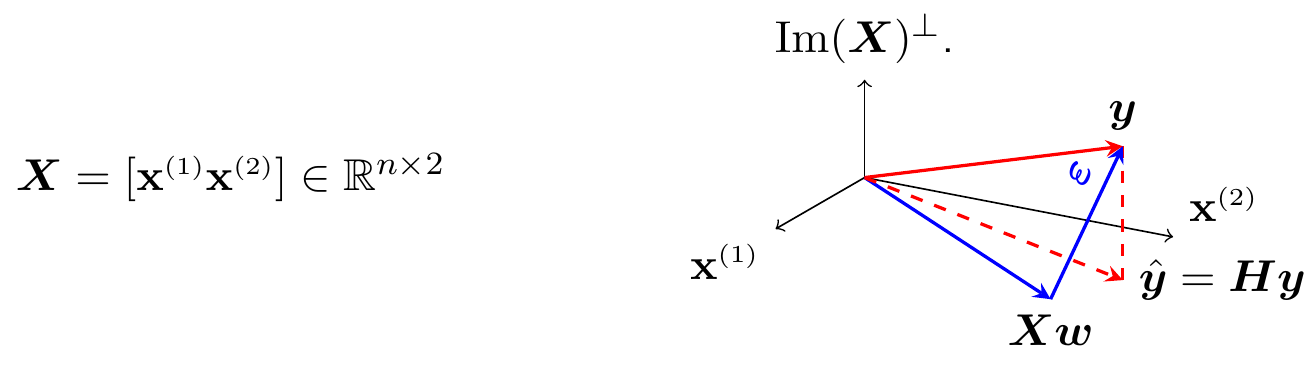
\includegraphics[scale=.2]{figures/geometry_linearRegression.png}}
\caption{Geometry of linear regression}
\label{fig:linreg_geometry}
\end{figure}

\subsection*{Optimality of least squares linear regression}
Assuming that $y = X\beta + \varepsilon$ where $\operatorname{rank}(X) = p$ i.e. full rank matrix and \textit{decorrelated centered noise} $\mathbb{E}[\varepsilon] = 0; \text{  } \mathbb{E}[\varepsilon^\top \varepsilon] = \sigma^2I$.

\begin{theorem}
    Gauss-Markov Theorem: Assuming the previous statements, $\hat \beta = \left( X^\top X\right)^{-1} X^\top y$ is the \textit{best linear unbiased estimator} (BLUE). That is, for any other \textit{unbiased} estimator $\tilde{\beta}$ we have
    $$\operatorname{Cov}(\tilde \beta) = \operatorname{Cov} (\hat \beta) + K_{\tilde \beta}$$ where $K_{\tilde \beta}$ is a \textit{possitive semi-definite} matrix. 
\end{theorem}

\begin{remark}[Positive (semi)definiteness]
A symmetric matrix $M \in \mathbb{R}^{d\times d}$ is called
\begin{itemize}
  \item \emph{positive semidefinite (psd)} if
  \[
  z^\top M z \;\geq\; 0 \quad \forall z \in \mathbb{R}^d,
  \]
  written $M \succeq 0$.
  \item \emph{positive definite (pd)} if
  \[
  z^\top M z \;>\; 0 \quad \forall z \in \mathbb{R}^d\setminus\{0\},
  \]
  written $M \succ 0$.
\end{itemize}
Equivalently:
\begin{itemize}
  \item $M\succeq 0$ if and only if all eigenvalues of $M$ are nonnegative,
  \item $M\succ 0$ if and only if all eigenvalues of $M$ are strictly positive.
\end{itemize}
\end{remark}	


% ------------------------------------------------------------------------------
% Reference and Cited Works
% ------------------------------------------------------------------------------

\bibliographystyle{IEEEtran}
\bibliography{biblio.bib}

% ------------------------------------------------------------------------------

\end{document}
